\documentclass{standalone}
\usepackage{tikz}

\begin{document}
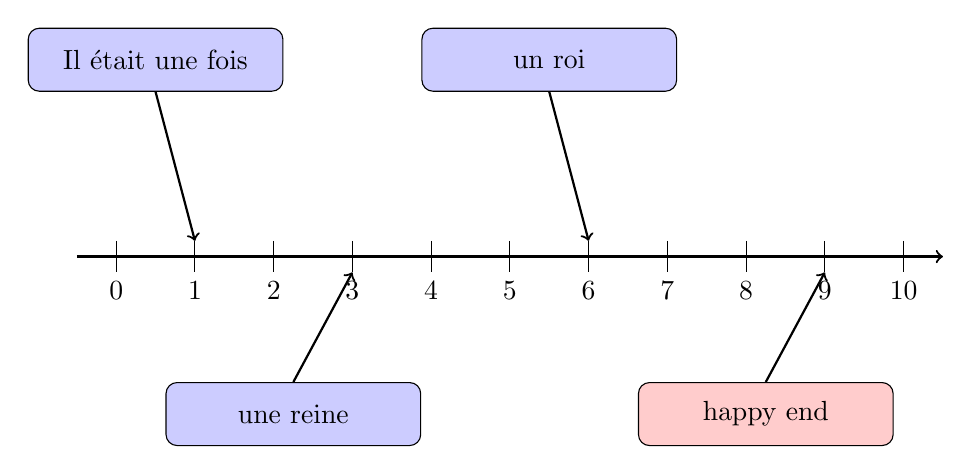
\begin{tikzpicture}
    \draw[->, thick] (-0.5, 0) -- (10.5, 0);
    \draw[-] (0, 0.2) -- (0, -0.2) node[below] {0};
    \draw[-] (1, 0.2) -- (1, -0.2) node[below] {1};
    \draw[-] (2, 0.2) -- (2, -0.2) node[below] {2};
    \draw[-] (3, 0.2) -- (3, -0.2) node[below] {3};
    \draw[-] (4, 0.2) -- (4, -0.2) node[below] {4};
    \draw[-] (5, 0.2) -- (5, -0.2) node[below] {5};
    \draw[-] (6, 0.2) -- (6, -0.2) node[below] {6};
    \draw[-] (7, 0.2) -- (7, -0.2) node[below] {7};
    \draw[-] (8, 0.2) -- (8, -0.2) node[below] {8};
    \draw[-] (9, 0.2) -- (9, -0.2) node[below] {9};
    \draw[-] (10, 0.2) -- (10, -0.2) node[below] {10};


    \node[
        rectangle,
        draw,
        fill=blue!20,
        rounded corners,
        minimum height=0.8cm,
        text width=3cm,
        align=center
    ] (fois) at (0.5, 2.5) {Il était une fois};

    \node[
        rectangle,
        draw,
        fill=blue!20,
        rounded corners,
        minimum height=0.8cm,
        text width=3cm,
        align=center
    ] (reine) at (2.25, -2) {une reine};

    \node[
        rectangle,
        draw,
        fill=blue!20,
        rounded corners,
        minimum height=0.8cm,
        text width=3cm,
        align=center
    ] (roi) at (5.5, 2.5) {un roi};

    \node[
        rectangle,
        draw,
        fill=red!20,
        rounded corners,
        minimum height=0.8cm,
        text width=3cm,
        align=center
    ] (fin) at (8.25, -2) {happy end};

    \draw[->, thick] (fois.south) -- (1, 0.2);
    \draw[->, thick] (roi.south) -- (6, 0.2);
    \draw[->, thick] (reine.north) -- (3, -0.2);
    \draw[->, thick] (fin.north) -- (9, -0.2);

\end{tikzpicture}
\end{document}